\chapter{Fabrication d'un transistor moléculaire}

\section{Lithographie optique}
La lithographie se déroule en deux étapes et vise à produire les éléments de grande taille telle les plots de connexion et les lignes d'amené, ainsi que la grille. Pour ces deux premières étape, une méthode bi-couche à base de LOR3A et de UV3 a été mise au point. Elle a l'avantage de prévenir la formation de bord lors de l'étape de lift-off~(cf Fig.\ref{lift-off}) qui pourrait entraîner une perte de contact entre la grille et le plot correspondant lors du passage de marche.

La première étape de lithographie vise tout d'abord à fabriquer les plots d'or nécessaire à la micro-soudure de notre échantillon ainsi que les lignes d'amené de courant~(cf partie orange de la Fig.\ref{LithoOptique}). La recette du Tab.\ref{tab_recette}  est utilisée pour obtenir un dép\^ot de 100$\,nm$ d'or avec une couche d'accroche en titane. Cette première étape nous permet également d'obtenir les marques d'alignements pour la fabrication de la grille. Une première série de marque (cf carré bleu de la Fig.\ref{LithoOptique}) permet d'effectuer un alignement grossier. Ce dernier est ensuite affiné à l'aide d'un seconde série de marques~(cf carré vert de la Fig.\ref{LithoOptique}).


\begin{figure}
\parbox{6.5cm}{
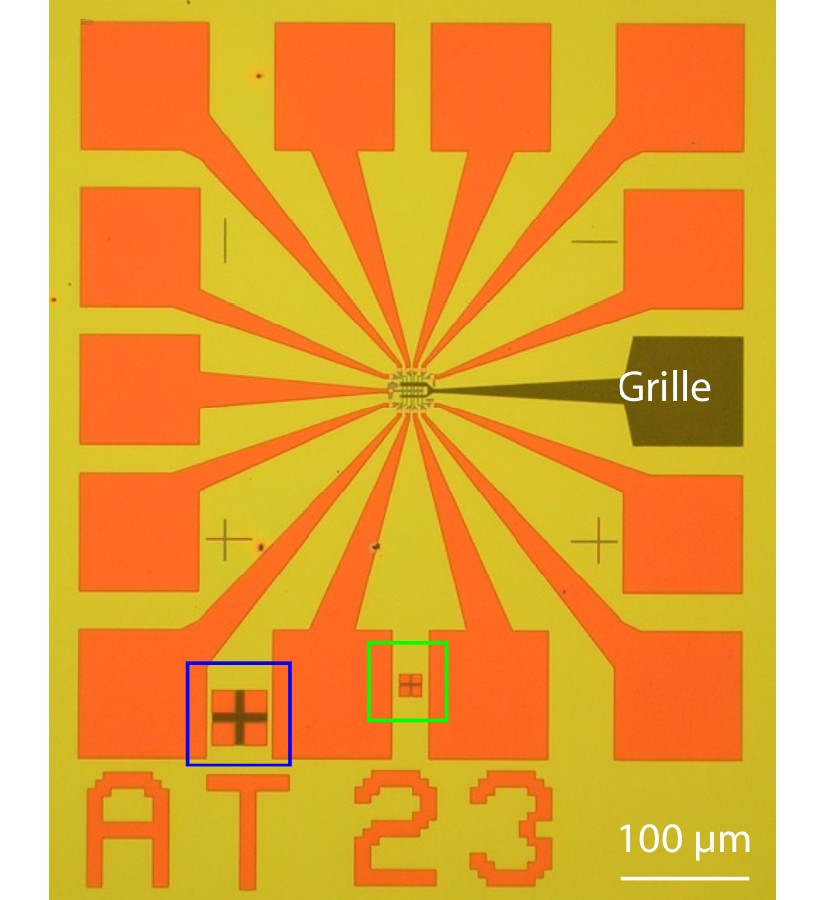
\includegraphics[scale=0.45]{Fabrication/LithoOptique/LithoOptique.pdf} 
}
\parbox{7cm}{\caption{Echanillon après les deux étapes de lithographie optique. Les lignes d'amené de courant sont visible en orange et la grille locale en gris. Les deux carrés repèrent les marque d'alignement. ~(extrait de la thèse de Nico)}
\label{LithoOptique}
}
\end{figure}

La seconde étape permet d'obtenir la grille locale de notre dispositif. La méthode présentée dans le Tab.\ref{tab_recette} est également utilisé avec pour seule différence l'épaisseur d'or déposée : $20\,nm$. Le résultat final est présenté dans la Fig.\ref{LithoOptique} où la partie orange désigne les lignes d'amené de courant et la partie grise la grille locale. La partie centrale, encore vide, va venir accueillir les nanofils d'or comme nous allons le voir dans la suite.


\begin{table}
\begin{center}
\begin{tabular}{|p{0.5cm}|p{4cm}|p{4cm}|p{3cm}|}
  \hline
\,& \textbf{étape} & \textbf{procédé} & \textbf{paramètres} \tabularnewline
\hline
1 &  nettoyage du wafer & acétone, ethanol, isopropanol et plasma oxygène (RIE)& $2\,$min \tabularnewline
\hline
 2 & étalement de LOR 3A pour une épaisseur de $400\,$nm& tournette & v\,:\,$2000\,$tr.min$^{-1}$, a\,:\,$2000\,$tr.min$^{-2}$, t\,:\,$30\,$s \tabularnewline
\hline
 3 & cuisson & plaque chauffante & $1\,$min à $170\,\degres$C \tabularnewline
\hline
4 & étalement de UV3 & tournette & v\,:\,$4000\,$tr.min$^{-1}$, a\,:\,$2000\,$tr.min$^{-2}$, t\,:\,$30\,$s \tabularnewline
\hline
5 & cuisson & plaque chauffante & $1\,$min à $130\,\degres$C \tabularnewline
\hline
6 & insolation & aligneur dUV MJB3 & $5.5\,$s à $0.3\,$mW.cm$^{-2}$\tabularnewline
\hline
7 & recuisson & plaque chauffante & $1\,$min à $130\,\degres$C \tabularnewline
\hline
8 & développement & MF-CD-26 & $30-40\,$s\tabularnewline
\hline
9 & neutralisation du développeur & eau DI & $1\,$min\tabularnewline
\hline
10 & dépôt de la couche d'accroche métallique & évaporateur à canon à électron PLASSYS & $5\,$nm de Ti à $0.1\,$nm.s$^{-1}$ \tabularnewline
\hline
11 & dépôt de la couche métallique principale & évaporateur à canon à électron PLASSYS & $100\,$nm de Au à $0.1\,$nm.s$^{-1}$ \tabularnewline
\hline
12 & \textit{lift-off} & acétone & $10\,$min à $1\,$h, on peut l'assister par ultra-son à $80\%$ de la puissance maximum. \tabularnewline
\hline
 13 & dissolution de LOR3A & PG-Remover & $1\,$h à $80\,\degres$C \tabularnewline
\hline
14 & rinçage & acétone et isopropanol & $1\,$min de chaque sous la pissette\tabularnewline
\hline
15 & séchage & azote sec & wafer posé sur du papier absorbant, pistolet à la verticale du wafer, ne pas toucher le wafer avec des pinces\tabularnewline
\hline
16 & nettoyage & plasma oxygène (RIE)& $10\,$min\tabularnewline
\hline
\end{tabular}
\caption{Recette du double couche LOR3A/UV3 : celle-ci permet de ne plus avoir d'effet de bord lors des lift-off.}
\label{tab_recette}
\end{center}
\end{table}






\section{Réalisation d'une grille locale}
La grille est un élément essentiel du transistor et c'est également vrai d'un transistor moléculaire. Dans ce dernier cas, elle permet notamment de moduler le potentiel chimique de la molécule allant jusqu'à modifier son état de charge~(cf annexe sur le transport mésoscopique). Elle permet également de contrôler la conductance du système~(avec le concours de la tension source-drain) ce qui permet de choisir des points de fonctionnement adaptés, comme nous le verrons dans la partie résultat. 

L'efficacité intrinsèque d'une grille peut être résumé en un critère : la charge induite. Celle-ci s'exprime simplement par $Q = CV_g^{max}$ où $Q$ est le charge induite et $C$ est la capacité associée à la grille, $V_g^{max}$ étant la tension maximale applicable à la grille. Un dernier élément importe également : la proximité de la grille avec la molécule composant le transistor. Plus celle-ci est proche, plus son efficacité est maximisée. Nous allons voir ceci à travers quelques exemples de grille mise en oeuvre dans différentes expériences. Puis nous présenterons notre technique de fabrication en introduisant notamment le dêpot par couche atomique~(ALD - Atomic Layer Deposition).

\subsection{Quelques exemples}
Si l'on exclue les grilles non-locales, on peut identifier trois géométries possibles : la grille au-dessus ou  ``\textit{top-gate}'', la grille latérale et la grille arrière ou  ``\textit{back-gate}''.

\subsubsection{La ``\textit{top-gate"}}
Cette configuration est celle utilisé dans l'industrie en ce qui concerne les transistors à effet de champ conventionnels. On la retrouve également dans les dispositifs expérimentaux faisant appel à des nanofils ou bien encore à des nanotubes. Elle a également pu être implémenté dans le cas de nanotubes suspendus donnant des résultats plus que convaincant.

Cette configuration est cependant difficilement compatible avec l'électromigration. En effet, dans ce cas, le gap formant la source et le drain se fait après les étapes de lithographie. Ceci serait impossible si le fil d'or était recouvert par une grille avant électromigration.

\subsubsection{La grille latérale}
Cette configuration consiste à placer la grille latéralement vis à vis du gap obtenu par électromigration. De plus, accompagné d'une ``Back-Gate", elle permet d'avoir un moyen supplémentaire de faire varier le potentiel chimique de la molécule située dans la gap. Il est en revanche très difficile de contr\^oler précisement la position de cette grille et elle se trouve donc souvent situé à plusieurs dizaine de nanomètre du gap. De plus, le r\^ole de l'oxyde est dans ce cas joué par l'air qui possède une permittivité de l'ordre de l'unité. Ceci a pour conséquence de diminuer fortement le couplage de la grille.


\subsubsection{La grille arrière}
Dans cette configuration, la grille se situe sous le dispositif. C'est cette configuration qui a été choisie lors de la fabrication du premier transistor à molécule unique. Elle est bien s\^ur compatible avec l'électromigration et c'est d'ailleurs cette configuration que nous avons également choisi d'adopter. La fabrication de cette dernière est grandement facilité par l'utilisation de la technique ALD que nous allons présenter dans la suite.

\begin{figure}
\centering 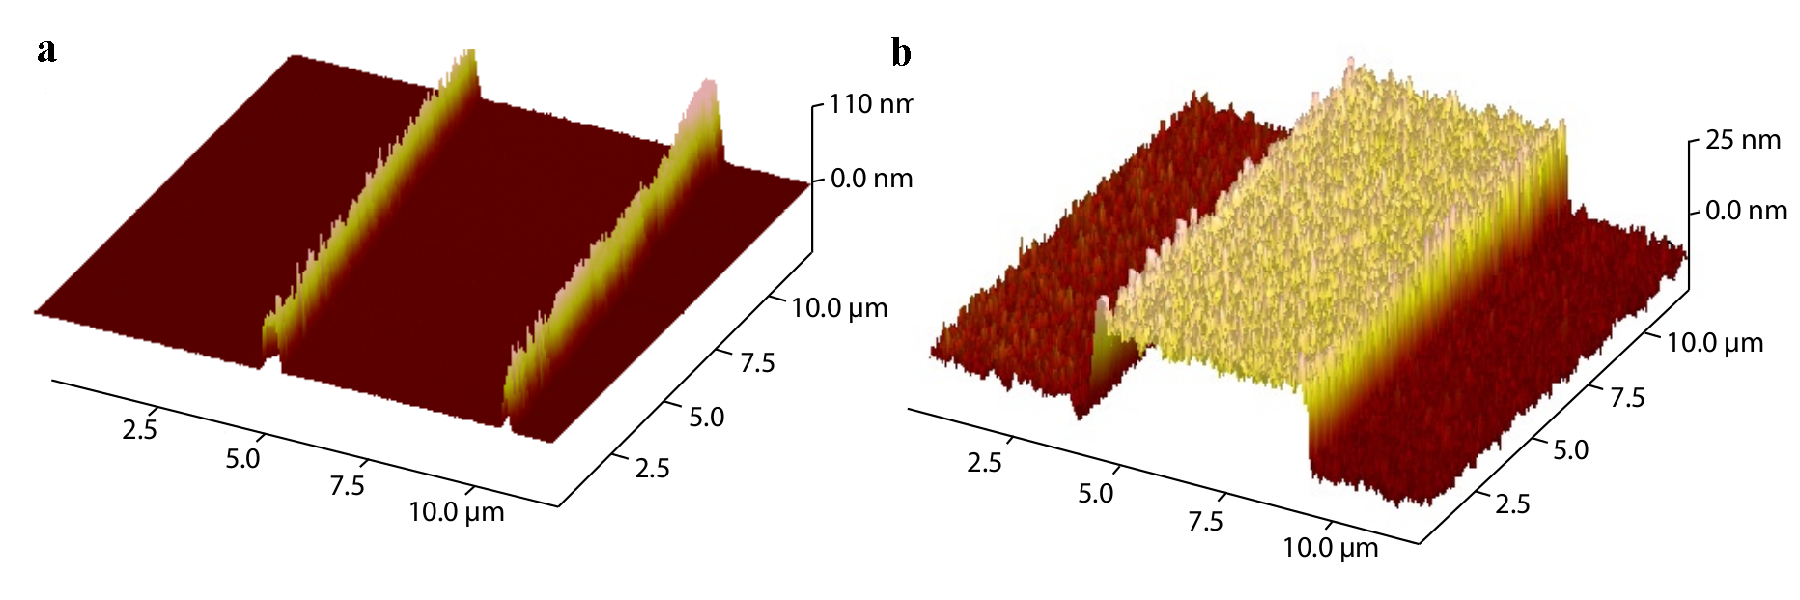
\includegraphics[scale=0.45]{Fabrication/BatmanGrille/BatmanGrille.pdf}
\caption{\textbf{a} : image AFM présentant des bords trop relevé d\^u à un problème de lift-off. \textbf{b} : image AFM montrant une grille n'ayant pas eu de problème de lift-off (extrait de la thèse de Nico).}
\label{lift-off}
\end{figure}



\subsection{Le choix de l'oxyde}
Dans la section précédente, nous avons aborder les différentes géométrie possible ainsi que les avantages et les inconvénients de chacune d'elles. L'aspect géométrique n'est pas le seul paramètre impliqué dans l’efficacité de la grille. Le choix de l'oxyde est également très important et pour que le couplage soit maximum, la permittivité de ce dernier doit être la plus élevée possible.

Parmis les oxydes à haute permittivité, l'alumine~($\kappa=8$) et l'hafnia~($\kappa=25$) sont parmis les plus utilisés. De manière générale, le premier est obtenue par dépôt d'une électrode d'aluminium, puis exposition à une atmosphère riche en oxygène. C'est d'ailleurs cette technique qui était en usage lorsque je suis arrivé en thèse. Bien que facile à mettre en œuvre, il est difficile de connaître avec exactitude l'épaisseur d'oxyde. De plus, nous avons observé une grande variabilité dans la qualité des grilles obtenue par ce procédé. Nous avons donc développer un nouveau procédé en utilisant une méthode de déposition par couche atomique~(ALD), nous permettant d'obtenir une grille avec un hafnia de $8\,nm$ environs.


\subsection{Le dép\^ot par ALD}
La technique d'ALD originellement appelée ALE~(pour Atomic Layer Epitaxie) a été breveté dans les années 1970~(référence du brevet+revue anguewante) et remise au goût du jour par les besoin toujours plus exigeant de la microélectronique. Elle consiste à une succession de deux réaction auto-limitante, aboutissant à la formation d'un oxyde.Une description détaillée est donnée dans la Fig.\ref{ALD}.

\begin{figure}
\centering 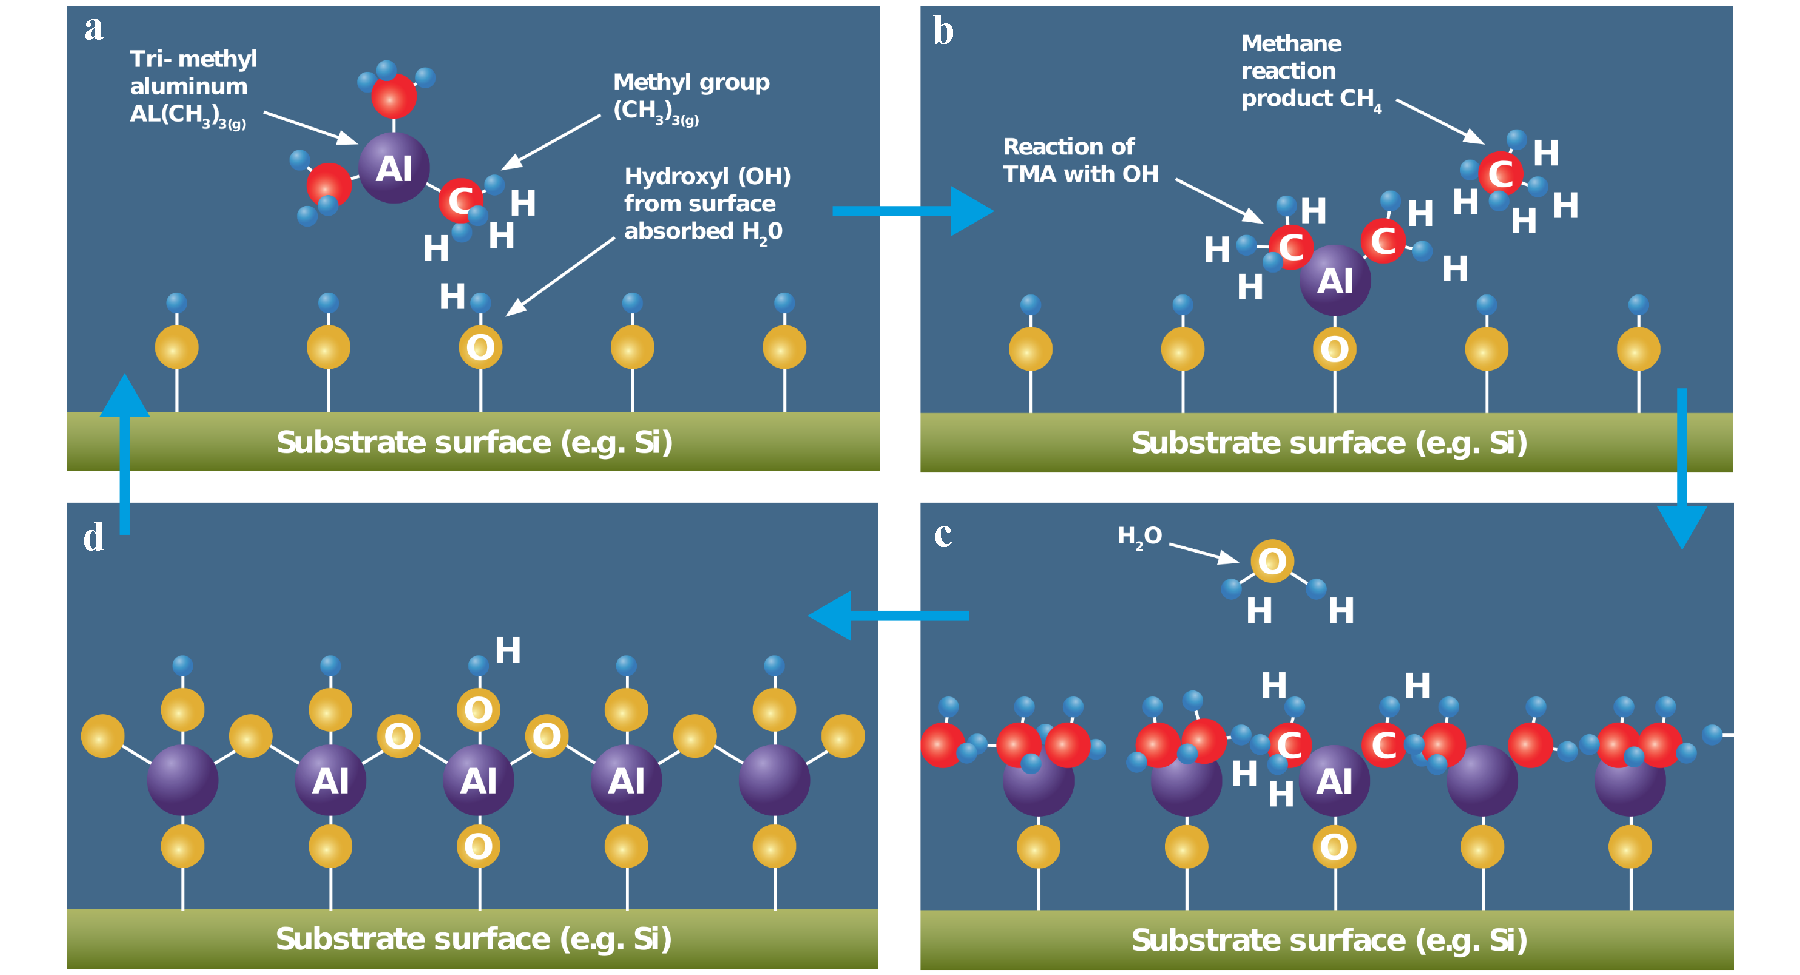
\includegraphics[scale=0.45]{Fabrication/ALD/ALD.pdf}
\caption{Première étape du cycle ALD : le premier précurseur, ici du Al(CH$_3$)$_{3(g)}$, se fixe à la surface~(\textbf{a}) et le produit issue la réaction de fixation sont évacués par un flux de gaz inerte~(\textbf{b}). Dans un deuxième temps, de l'eau est injecté et réagi avec la première couche de précurseur~(\textbf{c}) pour former une couche atomique d'oxyde~(\textbf{d}). Le cycle se répère ensuite à raison d'une couche atomique par cycle. (extrait du site CambrigeNanoTech)}
\label{ALD}
\end{figure}


Le premier avantage de la technique est sa facilité de mise en œuvre. Le contrôle du procédé, couche par couche, permet de choisir l'épaisseur d'oxyde avec une grande précision. De plus, le type d'oxyde est seulement déterminé par les précurseurs, ce qui donne un large choix.

En ce qui nous concerne, après quelques tests sur l'alumine, nous avons choisi de nous orienter sur un oxyde d'hafnium ou hafnia car ce dernier offre une permitivité plus élevé et donc un meilleur couplage. Ceci n'est cependant vrai que si la tension que l'on peut appliqué sur notre grille reste du même ordre de grandeur que celle utilisé avec les grille d'alumine, à savoir quelques volts. Pour cela, nous avons identifié deux qualité que devait avoir notre oxyde : peu d'impureté et être de préférence amorphe. 

Pour remplir le premier critère, l'idéal est de chauffer de façon suffisante le substrat afin de désorbé efficacement les déchet produit lors de la fixation du précurseur~(cf Fig.\ref{ALD}). La nature de ces dernier dépend du type de précurseur utilisé. Ce choix revet d'ailleurs une importance crucial car la qualité de l'oxyde varie grandement avec le choix des précursseurs et même de l'agent oxydant~(en général de l'eau ou de l'ozone). Pour certain application, une étape supplémentaire peut être inséré pour facilité la fixation des premières couches. C'est notamment le cas de nanotube ou une étape de fonctionnalisation à l'aide de NO$_2$ est nécessaire au bon déroulement de l'ALD.

Afin d'obtenir une structure amorphe, il est, au contraire, préférable d'effectuer le dép\^ot à basse température. Ceci a également l'avantage de rendre ce dernier compatible avec une étape de lithographie~(évitant à la résine de brûler). Il faut donc arriver à trouver un compromis avec ces deux conditions contradictoire.

Celui-ci été trouvé en laissant un temps conséquent entre les différentes étapes du dépôt, permettant aux produits de réaction de désorber. Cela se traduit par un temps d'attente entre chaque étape de cycle de 5 minutes. Un dépôt de $8\,nm$ d'hafnia prend donc un peu moins de six heures. Si ce temps peut paraître long au premier abord, il ne représente qu'un temps négligeable au regard des autres étapes et notamment de lithographie électronique que nous allons aborder maintenant.

\section{Réalisation d'un nanofil}
Comme nous l'avons présenté dans l'introduction, notre méthode de fabrication repose sur la technique d'électromigration. Cette dernière, pour fonctionner correctement, à besoin d'\^etre opérée sur des fils d'or très fins, présentant une section de quelque dizaine de nanomètre pour une épaisseur de quelque nanomètre en ce qui concerne la partie la plus fine~(cf Fig.\ref{EvapAngle}). 

\begin{figure}[h!]
\centering 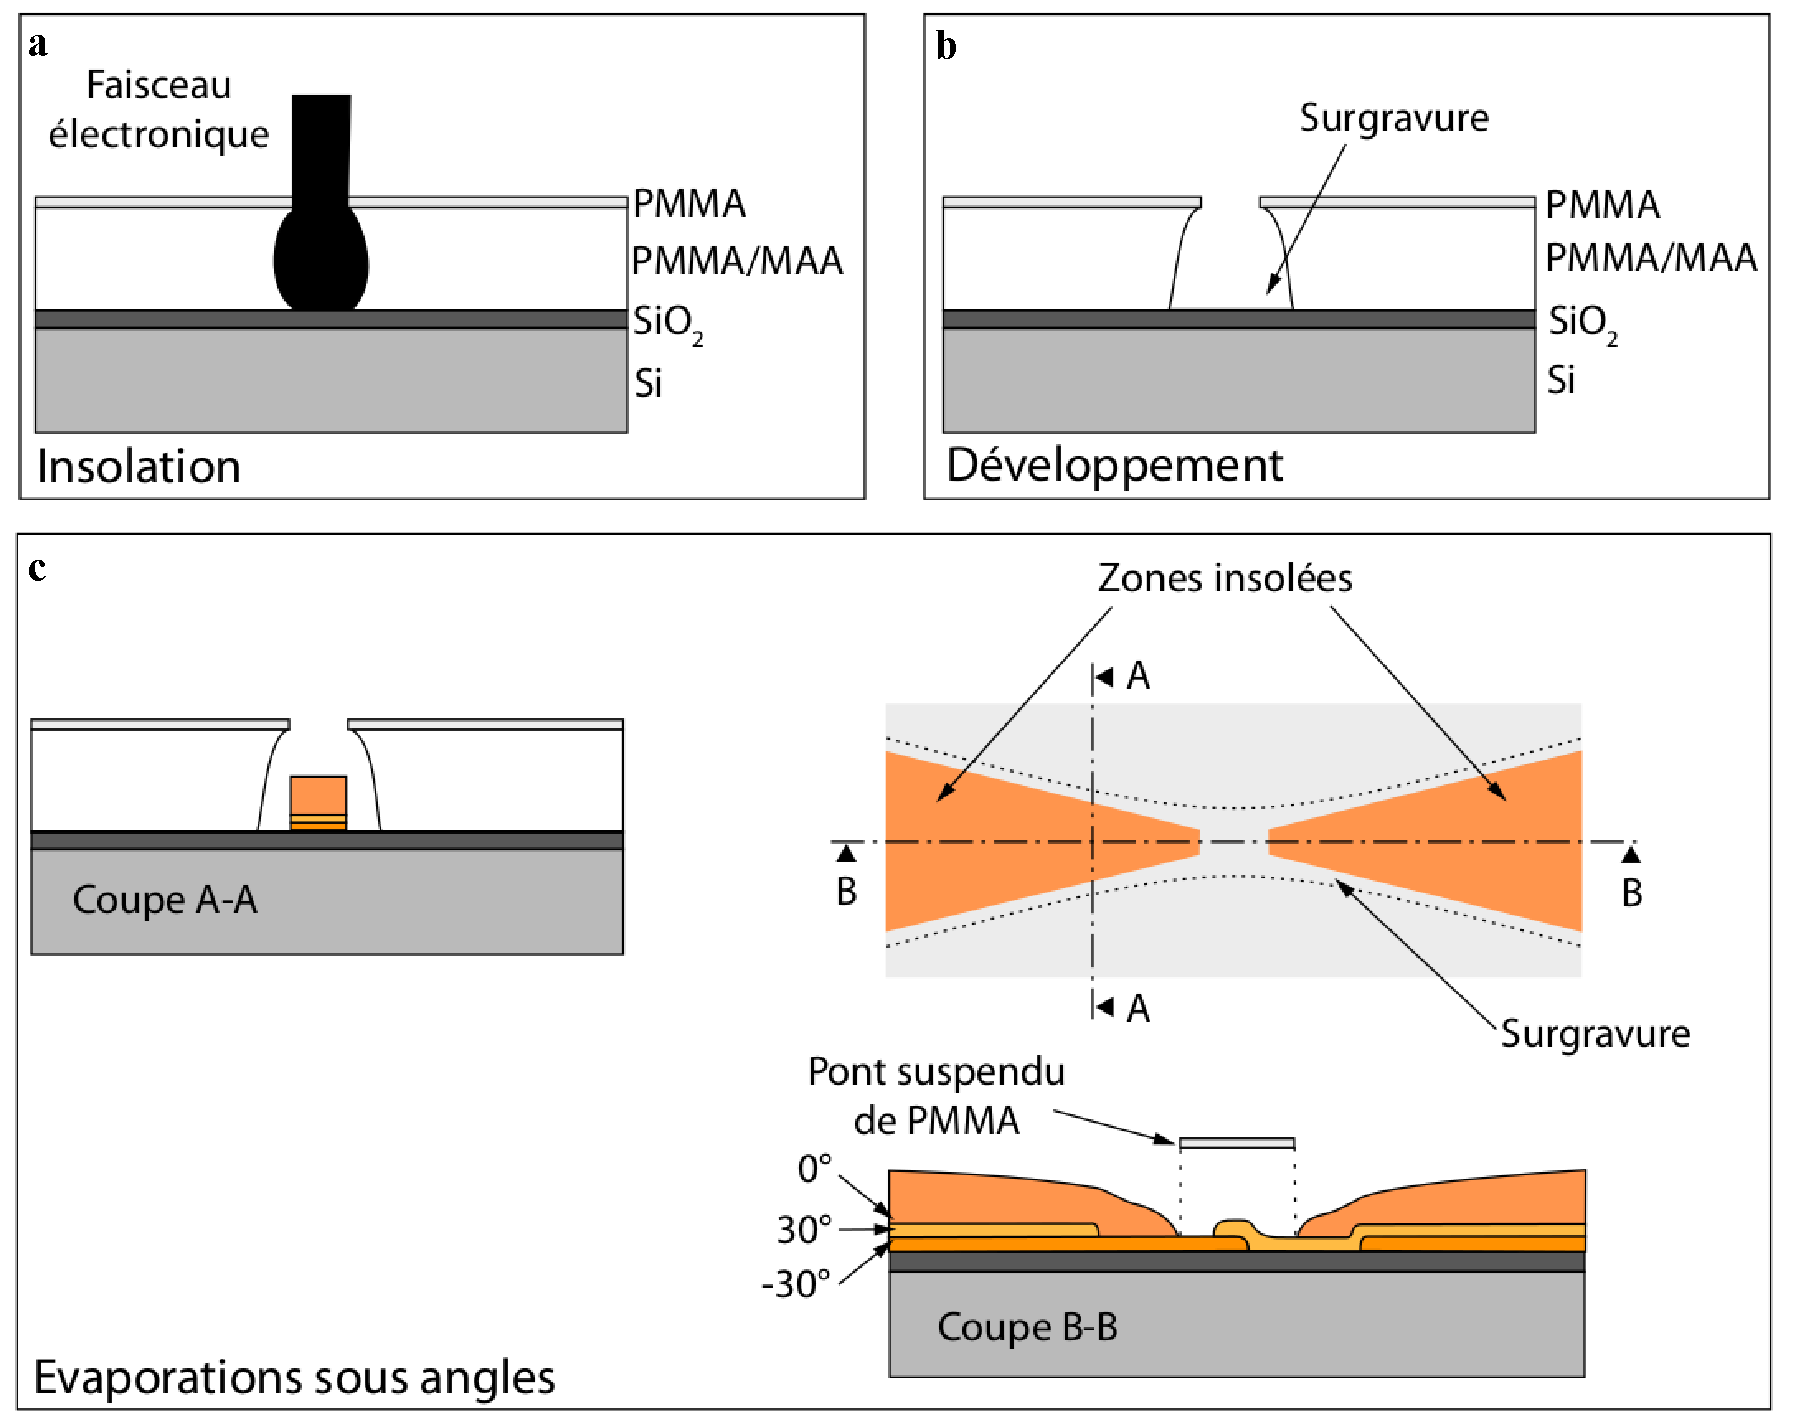
\includegraphics[scale=0.45]{Fabrication/EvapAngle/EvapAngle.pdf}
\caption{\textbf{a} : Insolation par lithographie électronique de la bicouche de résine. La partie la plus proche du substrat~(PMMA/MAA) se trouve plus insolé depart une plus grande sensibilité aux électrons et la présence des électrons rétrodiffusés. \textbf{b} : résultats après développement montrant clairement la surgravure généré par la surexposition de la partie basse. \textbf{c} : Evaporation sous angle : différentes couleurs représente les différents angle d'évaporation (-30$\,\degres$, 0$\,\degres$ et 30$\,\degres$). (extrait de la thèse de Nico).}
\label{EvapAngle}
\end{figure}

Le nanofil va également avoir un impact sur le couplage de la molécule à la grille. Cette dépendance se fait de deux manière. Tout d'abord, la forme de pointe donné au niveau de la partie fine du nanofilm va minimiser l'écrantage une fois le gap obtenue. Ensuite, en ayant une largeur faible, les films miniminise la surface en vis à vis avec la grille et donc le risque de fuit de grille à travers un défaut de l'oxyde, augmentant la tension maximale applicable.

Afin d'obtenir des fils répondant à ces critère, nous avons utilisé une méthode dite d'évaporation sous-angle. 

\begin{table}
\begin{center}
\begin{tabular}{|p{0.5cm}|p{4cm}|p{4cm}|p{3cm}|}
  \hline
\,& \textbf{étape} & \textbf{procédé} & \textbf{paramètres} \tabularnewline
\hline
1 &  dép\^ot de résine PMMA/MMA 2\,\% en masse & tournette & v\,:\,$6000\,$tr.min$^{-1}$, a\,:\,$4000\,$tr.min$^{-2}$, t\,:\,$30\,$s 
\tabularnewline
\hline
 2 & recuit (softbake) & plaque chauffante  & 5 minutes à 200$\, \degres C$ 
\tabularnewline
\hline
 3 & dépôt de résine PMMA 33\% en masse & tournette & v\,:\,$1400\,$tr.min$^{-1}$, a\,:\,$2000\,$tr.min$^{-2}$, t\,:\,$30\,$s \tabularnewline
\hline
4 & recuit & plaque chauffante & 5 minutes à 180$\, \degres C$
\tabularnewline
\hline
5 & insolation & MEB & dose de 350\,$\mu C.cm^{-2}$
\tabularnewline
\hline
6 & développement & becher MIBK/IPA (1:3) & 30 secondes
\tabularnewline
\hline
7 & rinçage & bécher IPA & 2 secondes
\tabularnewline
\hline
8 & surdéveloppement & bécher IPA & 1\,minute
\tabularnewline
\hline
9 & neutralisation du développeur &bécher d'eau désioninée & $1\,$minute\tabularnewline
\hline
10 & dépot de la couche d'accroche & évaporateur à canon à électron PLASSYS & $3\,$nm de Ti à $0.05\,$nm.s$^{-1}$, angle=$0\,\degres$
\tabularnewline
\hline
11 & dépôt de la constriction & évaporateur à canon à électron PLASSYS & $10\,$nm de Au à $0.1\,$nm.s$^{-1}$, angle=$\pm 30\degres$
\tabularnewline
\hline
12 &  dépôt des nanofils &  évaporateur à canon à électron PLASSYS  &  $100\,$nm de Au à $0.15\,$nm.s$^{-1}$, angle=$\pm 0\degres$
\tabularnewline
\hline
 13 & lift-off & bécher d'acétone & 1\,heure minimum 
\tabularnewline
\hline
14 & rinçage & acétone, éthanol et isopropanol & 
\tabularnewline
\hline
15 & séchage & azote sec & 
\tabularnewline
\hline
16 & nettoyage & plasma oxygène (RIE)& $3\,$min\tabularnewline
\hline
\end{tabular}
\caption{Recette du double couche PMMA/MAA : celle-ci permet d'obtenir des constrictions idéales pour l'électromigration.}
\label{tab_recette_elec}
\end{center}
\end{table}




Pour cela, il faut tout d'abord déposé deux couches de résine, la partie supérieur étant constitué de PMMA et la partir inférieur de PMMA-MAA, plus sensible aux électrons. On procède ensuite à la lithographie électronique puis au développement de la résine. Du fait de la plus grande sensibilité de la partie inférieure et la présence d'électron rétrodiffusés, on obtient une partie sur-insolé venant former un pont comme décrit sur la Fig.\ref{EvapAngle}.

On évapore ensuite une fine couche de titane~(5$\, nm$) avec un angle de $0\,\degres$ pour constituer un couche d'accroche. Puis on évapore, sous un angle de $\pm30\,\degres$, $10\, nm$ d'or  constituant la constriction. Enfin, $100\,nm$ d'or sont ensuite évaporé à $0\,\degres$ afin de venir relier la constriction aux plots de connexion. Cet épaisseur doit être également suffisant pour assurer un bon passage entre le partie se situant sur la grille et celle se trouvant sur la surface même du wafer. La structure finale est présenté dans la Fig.\ref{ZoomFinal}.

\begin{figure}
\centering 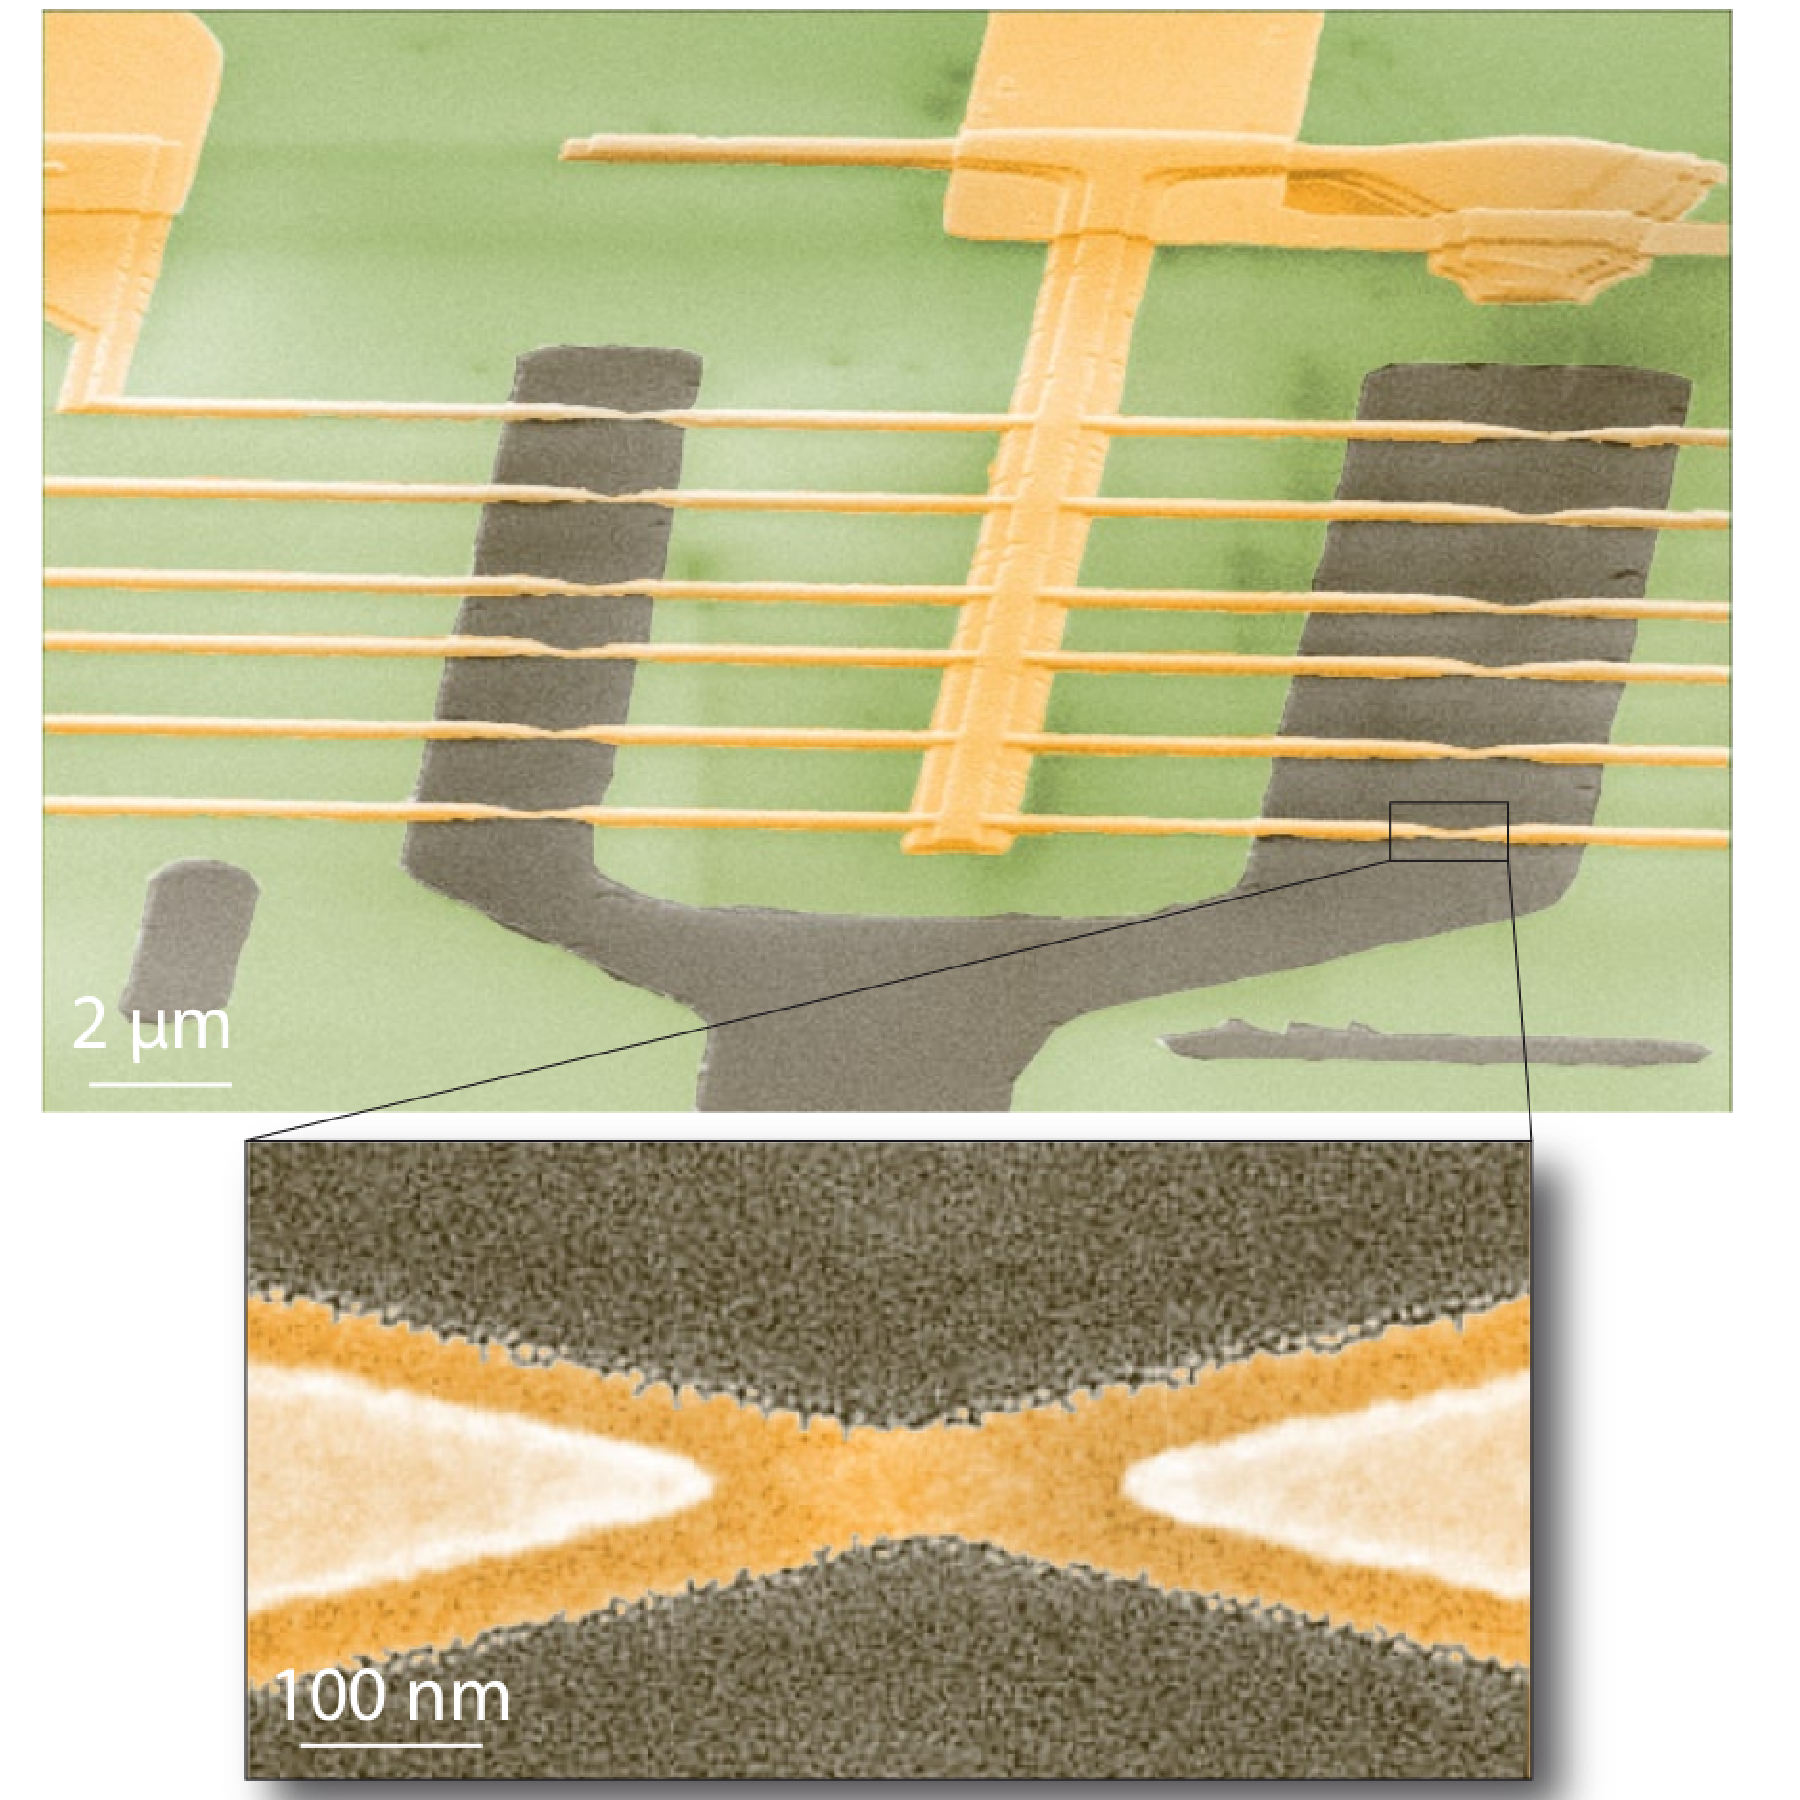
\includegraphics[scale=0.45]{Fabrication/ZoomFinal/ZoomFinal.pdf}
\caption{Image obtenu par microscopie électronique à balayage montrant la structure centrale de nos échantillons. Le grossissement présente une constriction obtenue à l'aide de l'évaporation sous angle. La grille, coloré en gris, est clairement visible au centre.}
\label{ZoomFinal}
\end{figure}


\section{Réalisation d'un interstice nanométrique}
Une fois que nous avons obtenue nos constriction métallique, il faut procéder à la dernière étape de fabrication : l'électromigration. Cette dernière, qui est effectué à basse température, va nous permettre d'obtenir les interstices de quelques nanomètres de largeur nécessaire à la fabrication d'un transistor moléculaire. Dans ce chapitre, nous présenterons dans un premier temps la technique d'électromigration ainsi que les différents méthode de sa mise en oeuvre. Nous finirons par une description de notre technique à basse température.

\subsection{L'électromigration}
L'électromigration est un phénomène connu depuis plus d'un siècle maintenant. Ce phénomène a connu un regain int\^eré avec le développement de la micro-électronique notamment parce qu'il a été identifié comme étant une cause de panne.

Le phénomène d'électromigration se produit lorsqu'une forte densité de courant traverse un conducteur. Les ions du réseau sont alors soumis à deux forces : la première est induite par le champ électrique induisant le courant, la seconde est d\^u aux électrons qui, du fait de la diffusion, viennent céder un peu de leur moment cinétique. L'action de ces deux forces de résume par la formule suivante :
\begin{eqnarray}
\textbf{F} = \textbf{F}_d + \textbf{F}_v = Z^*e\textbf{E} \nonumber
\end{eqnarray}
où $\textbf{F}_d$ est la force induite par le champ électrique et $\textbf{F}_v$ celle induite par la diffusion des électrons. Le terme $Z^*$ est en général utilisé pour représenté la charge effective des ions soumis à un champ électrique et rend compte de l'interaction ions/électrons.

Ce phénomène a été pour la première fois utilisé en électronique moléculaire par le groupe de D.C. Ralph à Cornell. La technique a notamment était mis en oeuvre pour réalisé le premier transistor à molécule unique. Depuis, la technique à connu de nombreuse évolution comme nous allons le voir maintenant

\subsection{Etat de l'art}
On peut classer les techniques d'électromigration en trois grande catégorie : a rampe unique, à contre-réaction et à cassure-spontanée (référence thèse de Stéphanie Girod).

\subsubsection{A rampe unique}
C'est la première technique qui a été mise en oeuvre dans le domaine de l'électronique moléculaire par Park \textit{et al.}(ref). Elle consiste en l'application d'une rampe de tension croissante sur une fin fil de métal. La simplicité de la méthode est séduisante mais mal contrôlé, elle peut conduire à une destruction de la jonction, notamment dû au chauffage induit par effet Joule.

\subsubsection{A contre-réaction}
Cette méthode à été développé par Strachan \textit{et al.} en 2005. Elle a pour but de réduire le chauffage de la jonction par effet Joule en introduisant une boucle de contre-réaction asservie sur la résistance de la jonction. Si celle-ci dépasse une valeur critique fixée à l'avance, la tension est diminué puis augmente à nouveau depuis une valeur plus basse. Ceci à pour effet de diminuer la puissance dissipé par la jonction lors de l'électromigration (voir figure). Le principal inconvénient de cette technique est son temps de mise en œuvre : la formation d'un seul gap peu prendre quelques heures.

\subsubsection{A cassure spontanée}
Cette dernière méthode a été mise au point dans le groupe de H.S.J. van der Zant en 2007. Une première étape d'électromigration contrôlée est d'abord réalisé à l'aide d'une méthode à contre-réaction. Lorsque la conductance du nanofil atteind une valeur de quelques kilo-Ohm. On laisse ensuité évoluer la jonction qui, du fait de l'instabilité de la nanoconstriction, va se rompre naturellement. On obtient ainsi un gap de quelques nanomètres. La durée d'une telle procédure varie d'un échantillon à l'autres : de quelques minutes à plusieurs heures.

\subsection{Notre technique}
Notre technique de fabrication a été développé à partir des travaux de Park \textit{et al.} puis améliorer en s'inspirant de travaux ultérieurs.

Afin d'augmenter de rendement de la méthode et la qualité des interstice obtenues, il a fallu apporter quelques modifications. Tout d’abord, la résitance en série avec la jonction à été diminué au maximum. Cela permet de limiter la puissance dissipé au niveau de la jonction et donc de mieux contrôler l'électromigration.

L'échelle de temps de l'électromigration est du domaine de la centain de $\mu s$. Afin de pouvoir contrôler parfaitement le déroulement du phénomène, il faut être capable d'agir sur ce dernier en un temps de l'ordre de la dizaine de $\mu s$. Ceci n'est possible que si la procédure d'électromigration se fait à l'aide d'une électronique en temps réel. Nous avons pour cela utilisé un ADWin contrôlé par un programme développé au sein du groupe. Grâce à ce dispositif, l'électromigration peut être détecté et la tension au borne de la jonction ramené à zéro dans un intervalle de $10\, \mu s$.

De plus, l'étape d'électromigration se fait à $4\,K$ et sous atmosphère hélium ce qui prévient la contamination de l'interstice au cours mais surtout après la procédure. De plus, nous pouvons analyser le dispositif directement après la procédure.


\section{Fabrication d'un transistor à molécule unique}
Pour obtenir un transistor moléculaire, il faut procéder selon trois étape. La première consiste en la réalisation d'un nanofil reposant sur une grille. On dépose ensuite les molécules sur la puce avant de la micro-soudé et de la disposé dans un frigo à dilution. Enfin, on procède à l'électromigration. Dans la partie précédente, nous avons aborder l'étape un et trois. Nous allons maintenant voir comment on dépose les molécules ainsi que la technique de caractérisation électrique des interstices.

\subsection{Dép\^ot des molécules}
Les cristaux de TbPc$_{2}$ sont dissous dans du dichlorométhane à la concentration 10$^{-6}mol.L^{-1}$. Une goute de la solution obtenue est ensuite déposé sur l'échantillon e t séché par un flux d'azote. L'échantillon obtenu est ensuite microsoudé sur l'échantillon, disposé dans un frigo à dilution et électromigré à basse température. Les jonctions obtenues (jusqu'à 12 par échantillons) sont ensuite analysé en transport.

\subsection{Les trois régimes de transport}
%\subsubsection{Couplage faible}
%\subsubsection{Couplage intermédiaire}
%\subsubsection{Couplage fort}
%\subsubsection{Présence de billes d'or}